\begin{figure}[t]
\begin{center}
%\includegraphics[width=0.29\textwidth, trim=0cm 0.5cm 0cm 0.5cm, clip]{figs/Fletcher.png}
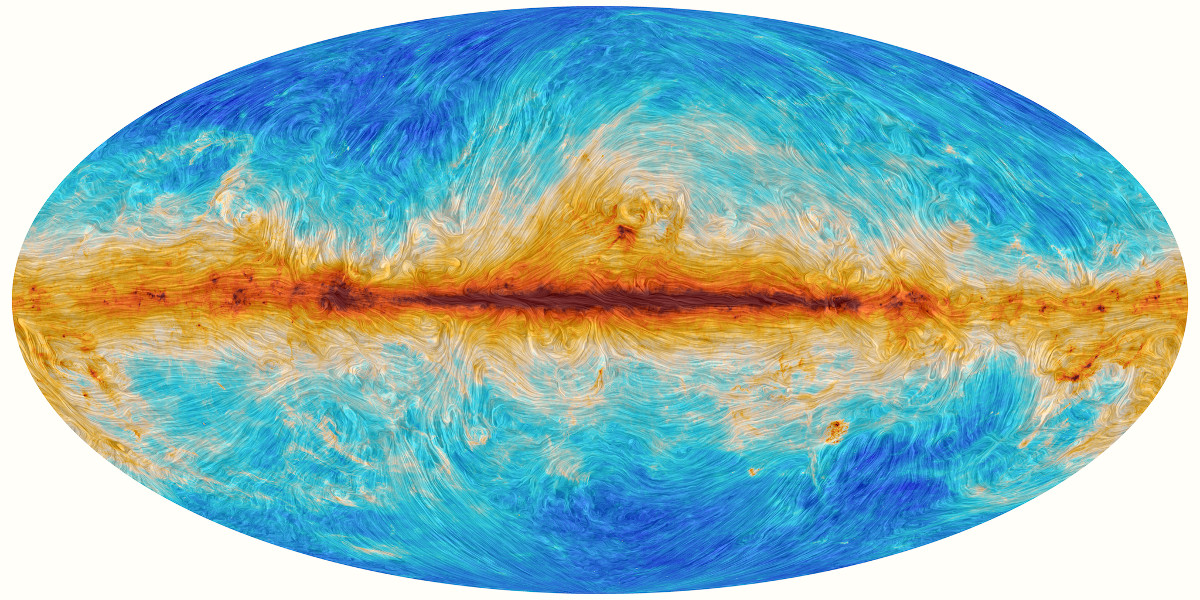
\includegraphics[width=0.65\textwidth, clip]{figs/Planck.jpg}
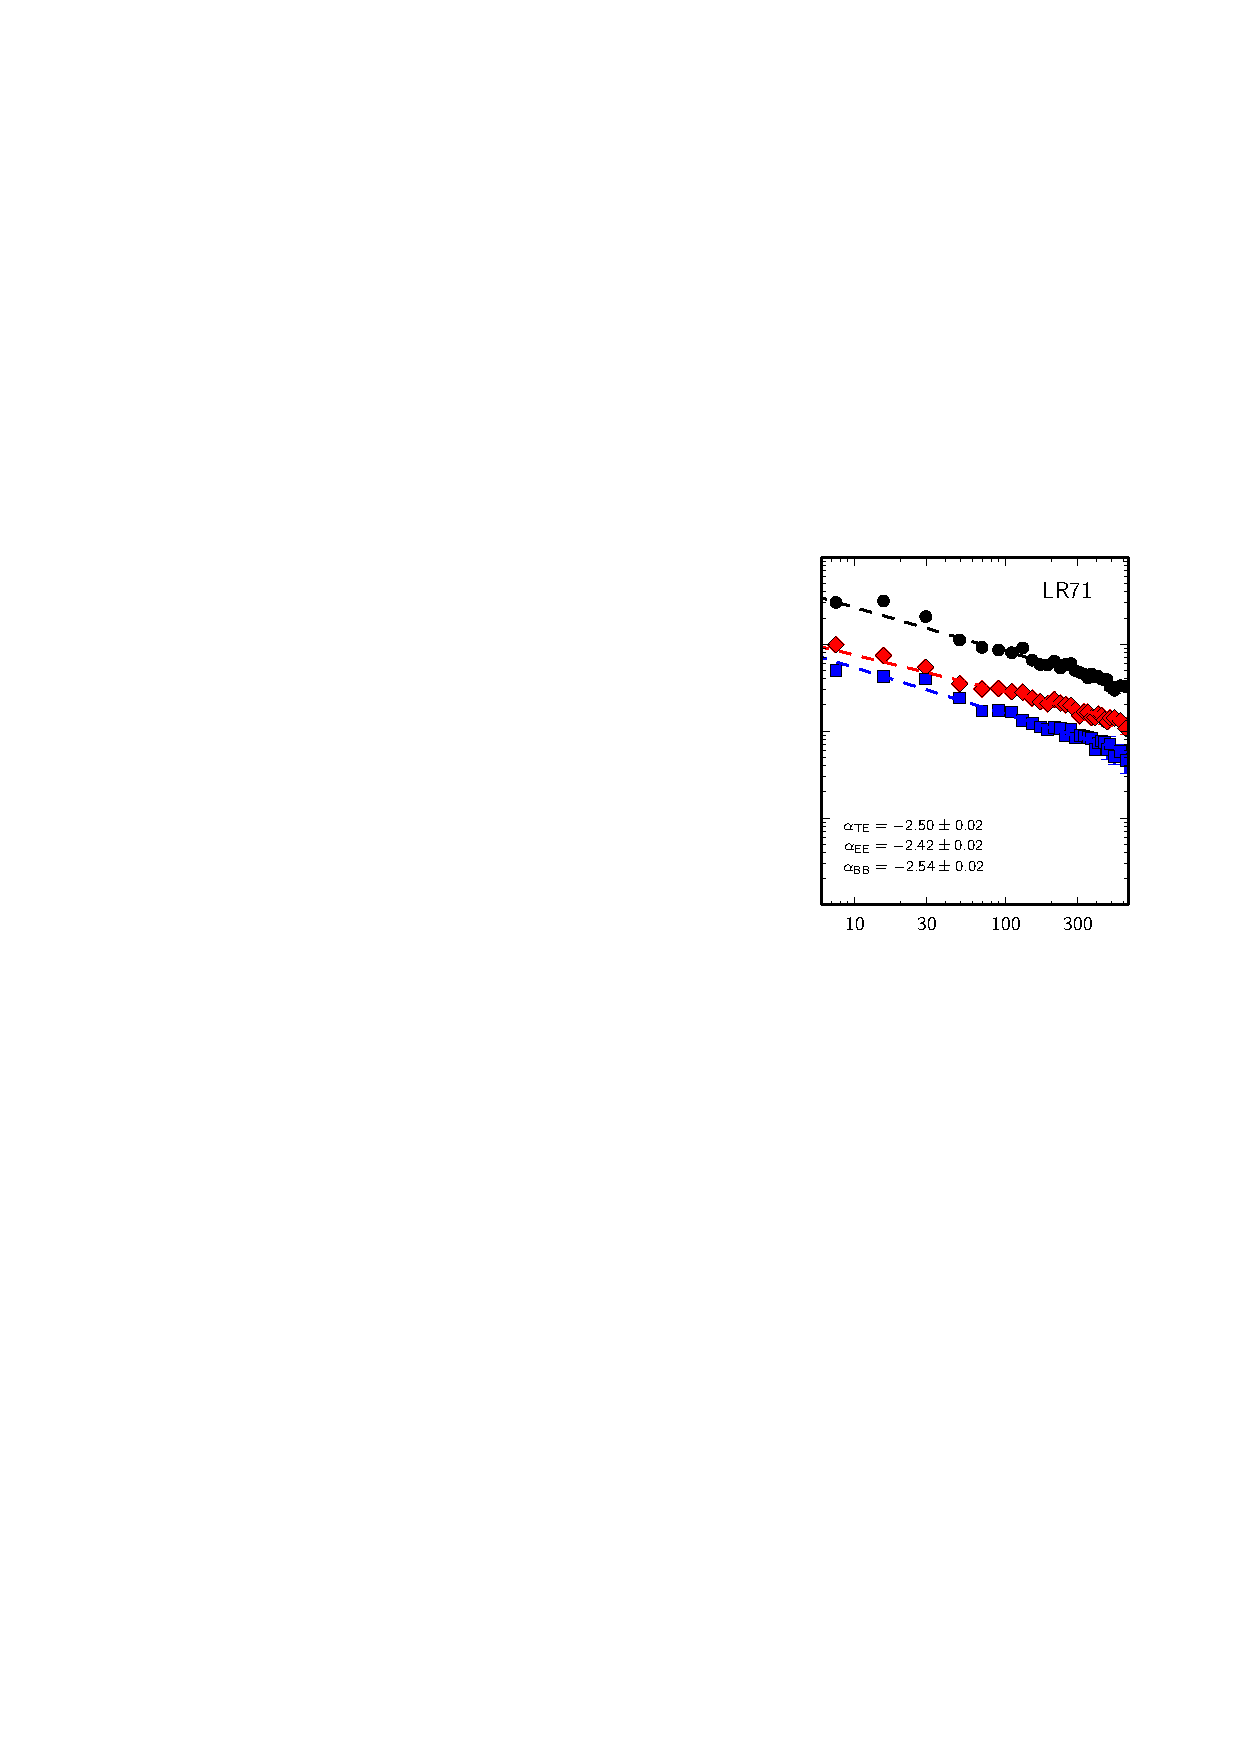
\includegraphics[width=0.27\textwidth, clip]{figs/PlanckForegrounds.pdf}
\end{center}
\vspace{-3mm}
\caption{\label{fig.planck} 
(\emph{Left}) The \emph{Planck} polarization map showing the 353 GHz dust
intensity convolved with the direction of polarization
\citep{PlanckIntermediateXIX15}.  This shows coherent structure on a range of
scales throughout the Milky Way.
(\emph{Right}) The spectrum of polarized emission from the sky, showing
$C_\ell^{TT}$ in
black, $C_\ell^{EE}$ in red, and $C_\ell^{BB}$ in blue.
}
%\vspace{-1mm}
\vspace{-4mm}
\end{figure}

